\documentclass{article}
\usepackage{amsmath}
\usepackage{enumitem}

\title{SECTION-A}
\author{}
\date{}

\begin{document}

\maketitle

\section*{Multiple Choice Questions}

\vspace{1em} % Adds vertical space

\textbf{Each question carries 1 mark.}



\begin{enumerate}
\item If $f(x) = 2x + 3$ and $f(1) = 1$, then $f(x)$ is
\begin{enumerate}
\item $x^2 + 3 \log |x| + 1$
\item $x^2 + 3 \log |x|$
\item $3$
\item $x^2 + 3 \log |x| - 4$
\end{enumerate}

\item Degree of the differential equation $\sin x + \cos (f) = y^2$ is
\begin{enumerate}
\item 2
\item 1
\item not defined
\item 0
\end{enumerate}

\item The integrating factor of the differential equation $(1 - y^2) \frac{dx}{dy} + yx = ay$, $(-1 < y < 1)$ is
\begin{enumerate}
\item $\frac{1}{1 - y^2}$
\item $\frac{1}{y^2 - 1}$
\item $\frac{1}{1 - y^2}$
\item $\frac{1}{y^2 - 1}$
\end{enumerate}

\item Unit vector along $\overrightarrow{PQ}$, where coordinates of $P$ and $Q$ respectively are $(2, 1, -1)$ and $(4, 4, -7)$, is
\begin{enumerate}
\item $\frac{2\hat{i} + 3\hat{j} - 6\hat{k}}{\sqrt{49}}$
\item $\frac{-2\hat{i} - 3\hat{j} + 6\hat{k}}{\sqrt{49}}$
\item $\frac{-2\hat{i} - 3\hat{j} + 6\hat{k}}{7}$
\item $\frac{2\hat{i} + 3\hat{j} - 6\hat{k}}{7}$
\end{enumerate}

\item If in $\triangle ABC$, $BA = 2\mathbf{a}$ and $BC = 3\mathbf{b}$, then $AC$ is
\begin{enumerate}
\item $2\mathbf{a} + 3\mathbf{b}$
\item $2\mathbf{a} - 3\mathbf{b}$
\item $3\mathbf{b} - 2\mathbf{a}$
\item $-2\mathbf{a} - 3\mathbf{b}$
\end{enumerate}

\item If $|\mathbf{a} \times \mathbf{b}| = \sqrt{13}$ and $\mathbf{a} \cdot \mathbf{b} = -3$, then angle between $\mathbf{a}$ and $\mathbf{b}$ is
\begin{enumerate}
\item $\frac{2\pi}{3}$
\item $\frac{\pi}{3}$
\item $\frac{5\pi}{6}$
\item $\frac{\pi}{6}$
\end{enumerate}

\item Equation of line passing through origin and making $30^\circ$, $60^\circ$, and $90^\circ$ with $x$, $y$, $z$ axes respectively is
\begin{enumerate}
\item $2x - \sqrt{3}y + z = 0$
\item $2x + \sqrt{3}y + z = 0$
\item $2x = \sqrt{3}y = z$
\item $2x - \sqrt{3}y - z = 0$
\end{enumerate}

\item If $A$ and $B$ are two events such that $P(A \cup B) = 2 \times P(B|A)$ and $P(A) + P(B) = \frac{3}{2}$, then $P(B)$ is equal to
\begin{enumerate}
\item $\frac{2}{9}$
\item $\frac{4}{9}$
\item $\frac{5}{9}$
\item $\frac{7}{9}$
\end{enumerate}

\item An antiderivative of $\tan^{-1}(\tan^{-1}x) + 1$ with respect to $x$ is
\begin{enumerate}
\item $\sec^2(x) + C$
\item $-\sec^2(x) + C$
\item $\log|\sec(x)| + C$
\item $-\log|\sec(x)| + C$
\end{enumerate}

\item If $(a, b)$, $(c, d)$, and $(e, f)$ are the vertices of $\triangle ABC$ and $\Delta$ denotes the area of $\triangle ABC$, then
\[
\begin{vmatrix}
a & c & e \\
b & d & f \\
1 & 1 & 1 \\
\end{vmatrix}
\]
is equal to
\begin{enumerate}
\item $2\Delta$
\item $4\Delta$
\item $2\Delta^2$
\item $4\Delta^2$
\end{enumerate}

\item The function $f(x) = x|x|$ is
\begin{enumerate}
\item continuous and differentiable at $x = 0$
\item continuous but not differentiable at $x = 0$
\item differentiable but not continuous at $x = 0$
\item neither differentiable nor continuous at $x = 0$
\end{enumerate}

\item If $\tan^{-1}\left(\frac{1}{x}\right) = k$, then $k$ is equal to
\begin{enumerate}
\item $\frac{\pi}{7}$
\item $\frac{\pi}{4}$
\item $\sec^2(x)$
\item $-\sec^2(x)$
\end{enumerate}

\item The objective function $Z = ax + by$ of an LPP has maximum value 42 at $(4, 6)$ and minimum value 19 at $(3, 2)$. Which of the following is true?
\begin{enumerate}
\item $a = 9, b = 1$
\item $a = 5, b = 2$
\item $a = 3, b = 5$
\item $a = 5, b = 3$
\end{enumerate}

\item The corner points of the feasible region of a linear programming problem are $(0, 4)$, $(8, 0)$, and $(2\frac{2}{3}, \frac{5}{3})$. If $Z = 30x + 24y$ is the objective function, then (maximum value of $Z$ - minimum value of $Z$) is equal to
\begin{enumerate}
\item 40
\item 96
\item 120
\item 136
\end{enumerate}

\item If $A$ is a $2 \times 3$ matrix such that $AB$ and $AB'$ both are defined, then order of the matrix $B$ is
\begin{enumerate}
\item $2 \times 2$
\item $2 \times 1$
\item $3 \times 2$
\item $3 \times 3$
\end{enumerate}

\item If $P = \begin{bmatrix} 2 & 5/2 \\ 5/2 & 4 \end{bmatrix}$ and $Q$ is a skew symmetric matrix, then $Q$ is equal to
\begin{enumerate}
\item $\begin{bmatrix} 2 & 5/2 \\ 5/2 & 4 \end{bmatrix}$
\item $\begin{bmatrix} 0 & 5/2 \\ -5/2 & 0 \end{bmatrix}$
\item $\begin{bmatrix} 5/2 & -5/2 \end{bmatrix}$
\item $\begin{bmatrix} 5/2 & -1/2 \end{bmatrix}$
\end{enumerate}

\item If $|A| = |kA|$, where $A$ is a square matrix of order 2, then sum of all possible values of $k$ is
\begin{enumerate}
\item 1
\item -1
\item 2
\item 0
\end{enumerate}
\section*{Assertion-Reason Based Questions}
\item[18.]In the following questions 19 \& 20, a statement of Assertion (A) is followed by a statement of Reason (R). Choose the correct answer out of the following choices:

\begin{enumerate}
\item[(A)] Both (A) and (R) are true and (R) is the correct explanation of (A).
\item[(B)] Both (A) and (R) are true, but (R) is not the correct explanation of (A).
\item[(C)] (A) is true, but (R) is false.
\item[(D)] (A) is false, but (R) is true.
\end{enumerate}

\begin{enumerate}
\item[19.] \textbf{Assertion (A):} If a line makes angles $\alpha$, $\beta$, $\gamma$ with the positive direction of the coordinate axes, then $\sin^2 \alpha + \sin^2 \beta + \sin^2 \gamma = 2$. \\
\textbf{Reason (R):} The sum of squares of the direction cosines of a line is 1.
\end{enumerate}
\section*{SECTION-B}

\textbf{This section comprises Very Short Answer Type (VSA) questions, each of 2 marks}.

\begin{enumerate}
\item[21.] If $\mathbf{a}$, $\mathbf{b}$, $\mathbf{c}$ are three non-zero unequal vectors such that $\mathbf{a} \cdot \mathbf{b} = \mathbf{a} \cdot \mathbf{c}$, then find the angle between $\mathbf{b}$ and $\mathbf{c}$.

\item[22.]
\begin{enumerate}
\item[(a)] Evaluate $\sin^{-1}(\sin\frac{3\pi}{4}) + \cos^{-1}(\cos \pi) + \tan^{-1}(1)$.

\item[(b)] Draw the graph of $\cos^{-1} x$, where $x \in [-1, 0]$. Also, write its range.
\end{enumerate}

\item[23.] If the equation of a line is $x = ay + b$, $z = cy + d$, then find the direction ratios of the line and a point on the line.

\item[24.]
\begin{enumerate}
\item[(a)] If $y = bx$, prove that $y \left(\frac{d^2y}{dx^2}\right) + \left(\frac{dy}{dx}\right)^2 = 0$.

\item[(b)] If $f(x) =
\begin{cases}
ax + b, & 0 < x < 1 \\
x^2 - x, & 1 < x \leq 2
\end{cases}$ is a differentiable function in $(0, 2)$, then find the values of $a$ and $b$.
\end{enumerate}

\item[25.] If the circumference of a circle is increasing at a constant rate, prove that the rate of change of the area of the circle is directly proportional to its radius.

\end{enumerate}
\section*{SECTION C}

\noindent This section comprises Short Answer (SA) type questions of 3 marks each.

\begin{enumerate}
\item[26.] Evaluate $\int \frac{\log x}{\log^2 3} \, dx$

\item[27.]
\begin{enumerate}
\item[(a)] Find the general solution of the differential equation: $(xy - x^2) \, dy = y^2 \, dx$.

\item[(b)] OR Find the general solution of the differential equation: $(x^2 + 1) + 2xy = y + 4$.
\end{enumerate}

\item[28.]
\begin{enumerate}
\item[(a)] Two balls are drawn at random one by one with replacement from an urn containing equal numbers of red balls and green balls. Find the probability distribution of the number of red balls. Also, find the mean of the random variable.

\item[(b)] OR A and B throw a die alternately till one of them gets a '6' and wins the game. Find their respective probabilities of winning, if A starts the game first.
\end{enumerate}

\item[29.] Solve the following linear programming problem graphically: Maximize: $Z = x + 2y$ subject to constraints: $x + 2y \leq 100$, $2x - y \geq 0$, $2x + y \leq 200$, $x \geq 0$, $y \geq 0$.

\item[30.]
\begin{enumerate}
\item[(a)] Evaluate $\int_{-1}^{1} |x^4 - x| \, dx$.

\item[(b)] OR Find $\int \frac{\sin^{-1} x}{(1 - x^2)^{3/2}} \, dx$.
\end{enumerate}

\item[31.] Find $\int \frac{e^x (1 - \sin x)}{1 - \cos x} \, dx$
\end{enumerate}
\section*{SECTION-D}
\textbf{This section comprises Long Answer type (LA) questions of 5 marks each}.

\begin{enumerate}
\item[(32)] (a) Find the equations of the diagonals of the parallelogram $PQRS$ whose vertices are $P(4, 2, -6)$, $Q(5, -3, 1)$, $R(12, 4, 5)$ and $S(11, 9, -2)$. Use these equations to find the point of intersection of diagonals. \hfill (5)
\textbf{OR}

(b) A line $l$ passes through point $(-1, 3, -2)$ and is perpendicular to both the lines $\frac{x}{1} = \frac{y}{2} = \frac{z}{3}$ and $\frac{x + 2}{1} = \frac{y}{-1} = \frac{z + 1}{5}$. Find the vector equation of the line $l$. Hence, obtain its distance from origin. \hfill (5)

\item[(33)] Using Integration, find the area of the triangle whose vertices are $(-1, 1)$, $(0, 5)$ and $(3, 2)$. \hfill (5)

\item[(34)] A function $f: [-4, 4] \to [0, 4]$ is given by $f(x) = x^2$. Show that $f$ is an onto function but not a one-one function. Further, find all possible values of $a$ for which $f(a) = 5$. \hfill (5)

\item[(35)] (a) If $A = \begin{bmatrix} -3 & -2 & -4 \\ 2 & 1 & 2 \\ 1 & 3 & 1 \end{bmatrix}$ and $B = \begin{bmatrix} 1 & 2 & 0 \\ -2 & -1 & -2 \\ 0 & -1 & 3 \end{bmatrix}$, then find $AB$ and use it to solve the following system of equations:
\[
\begin{aligned}
x - 2y &= 3 \\
2x - y - z &= 2 \\
-2y + z &= 3
\end{aligned}
\]
\hfill (5)

\textbf{OR}

(b) If $f(\alpha) = \begin{bmatrix} \cos \alpha & -\sin \alpha &  0 \\ \sin \alpha & \cos \alpha & 0 \\ 0 & 0 & 1 \end{bmatrix}$, then prove that $f(\alpha) \cdot f(-\alpha) = f(\alpha - \alpha)$. \hfill (5)
\end{enumerate}
\section {SECTION-E}
\textbf{This section comprises 3 source based case-based/passage based/integrated units of assessment questions of 4 marks each}
\item[36.]\text{Recent studies suggest that roughly 12\% of the world population is left handed}
	\begin{figure}
		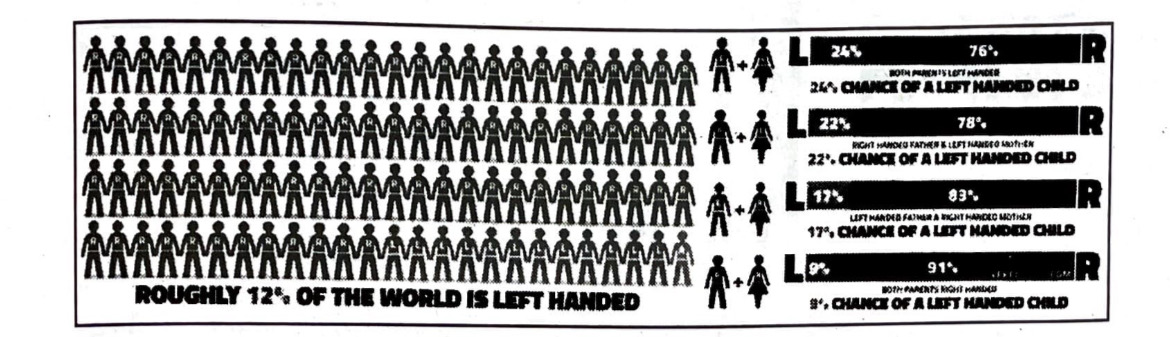
\includegraphics{IMG_9725.PNG}
	\end{figure}
Depending upon the parents,the chances of having a left handed child as folws;
\begin{itemize}
\item [A:] When both father and mother are left handed:\\
Chances of left handed child is 24%
\item [B:] When father is right handed and mother is left handed:\\
Chances of left handrd child is 22%
\item [C:] When father is left handed and mother is right handed:\\
Chances of left handed child is 17%
\item [D:] When both faher and mother are right handed ;\\
Chances of left handed child is 9%
\end{itemize}
Assuming that $P(A) = P(B) = P(C) P(D) =\frac{1}{4}$ and \(L\) denotes the event that child is left handed\\
\text{Based on the above information, answer the following questions:}
\item [(i)] Find \(P(L|C)\)
\item [(ii)] Find \(p(\overline{L}|A)\)
\item [(iii)](a) Find \(P(A|L)\)\\
OR\\
(b) Find the probability that a randomly selected child is left handed given that exactly one of the parents is left handed.
\item [37.] Engine displacement is the measure of the cylinder volume swept by all the pistons engine.The piston moves inside the cylinder bore \\
The cylinder bore in the form of circular cylinder open at the top is to be made from a metal sheet of area $75\pi cm^2$\\
\vspace{1em} % Adds vertical space

Based on the above information, answer the following questions:
\begin{itemize}
\item [(i)] if the radius of cylinder is "r" cm and height is "h" cm,then write the volume V of cylinder in terms of radius "r".
\item [(ii)] Find $\frac{dV}{dr}$.
\item [(iii)] (a) Find the radius of the cylinder when its volume is maximum.\\
OR\\
(b)For maximum volume, \(h>r\).State true or false and justify.
\end{itemize}
\item [38.] The use of electric vehicles will curb air pollutionin the long run.\\
The use of electric vechiles is incereasing every year and estimated electric vechiles in use at any time \(t\) is given by the function \(V\):\\
$V(t)=\frac{1}{5} t^3-\frac{5}{2}t^2+25t-2\\$
where \(t\) represents the time and t=1,2,3....corresponds to year 2001,2002,2003,...respectively.\\
Based on the above information, answer the following questions :
\begin{itemize}
    \item [(i)] Can the above function be used to estimate number of vechicles in the year 2000 ? Justify.
    \item [(ii)] Prove that the function \(V(t)\) is an increasing function.
    \end{itemize}

\end{enumerate}
\end{document}
